% TODO: scrivere discussione dello schema ER portante
% DONE: definire schema ER portante
\section{Schema E/R portante}
Analizzando le problematiche presentate si è arrivati all'individuazione delle
seguenti entità fondamentali:
\begin{description}
\item[Membro] Anagrafica dei membri dell'equipaggio
\item[Missione] Affidata dall'agenzia spaziale internazionale per l'esplorazione e analisi del
  terreno lunare
\item[Report] Report redatti dai membri sull'esito di una missione
\item[Robot] Una delle risorse utilizzabili in una missione
\item[Sensore] La risorsa principale utilizzata in una missione
\end{description}
\begin{figure}
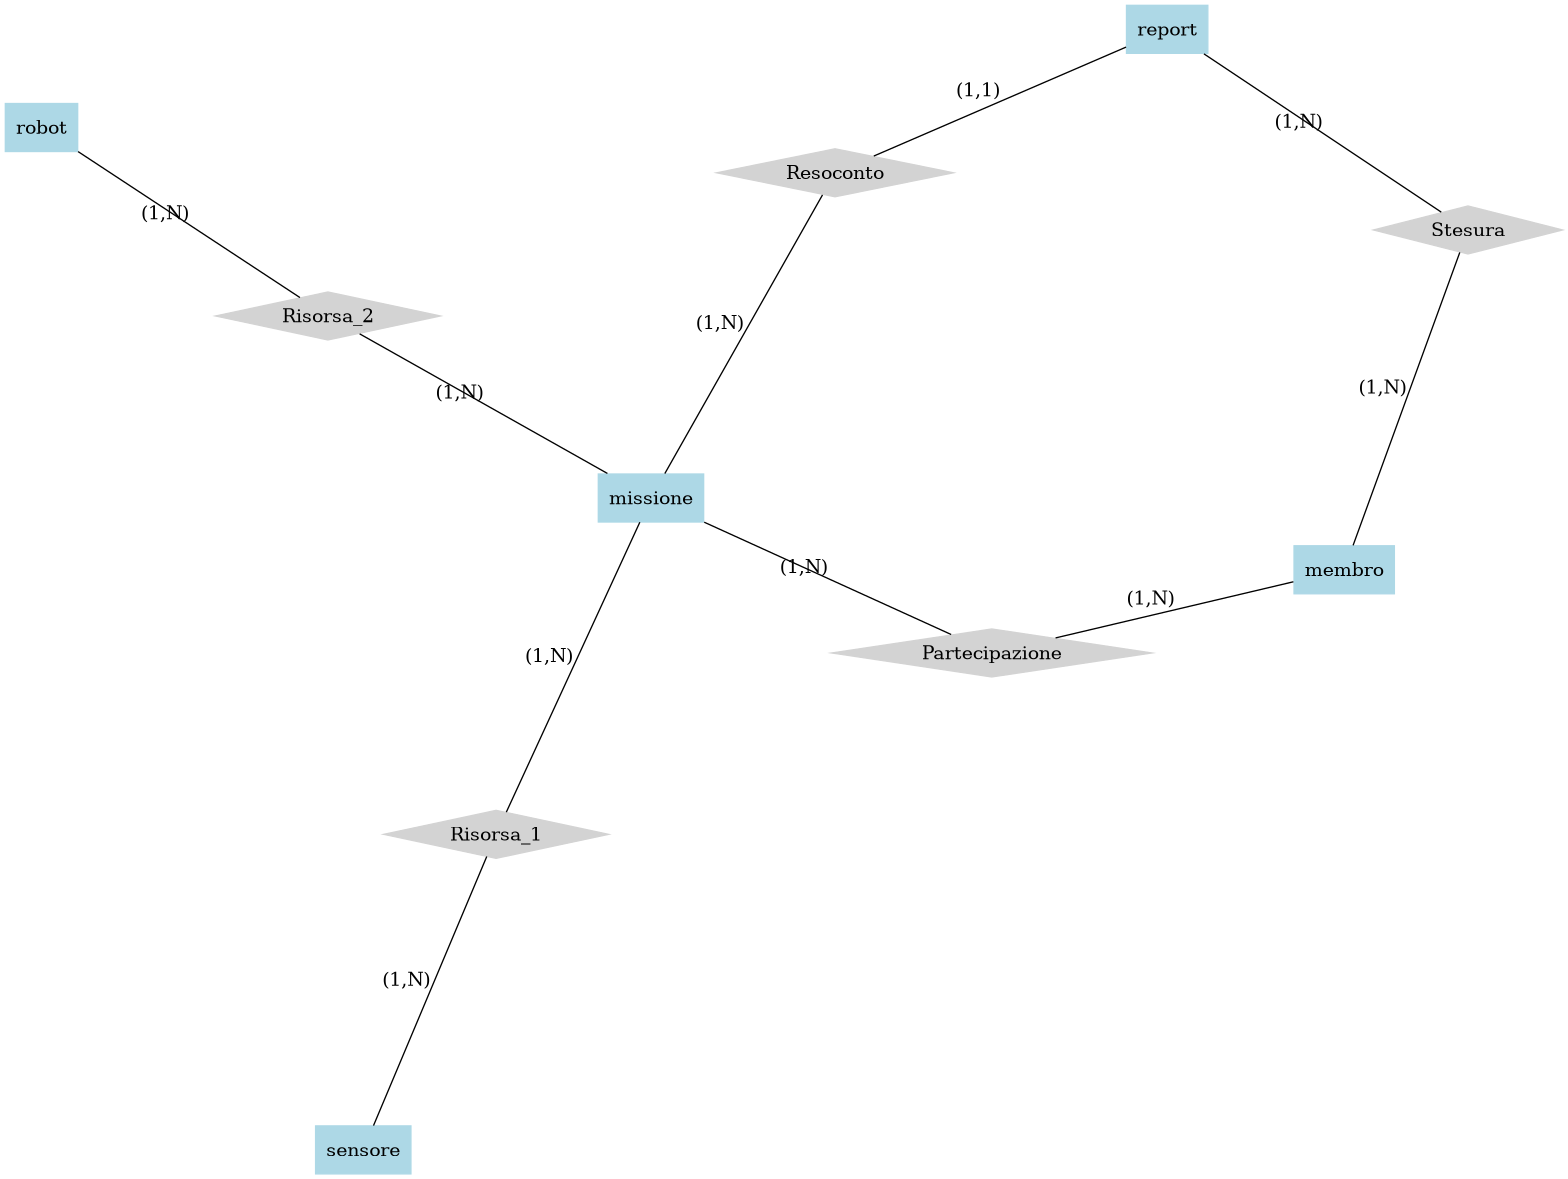
\includegraphics[width=\linewidth]{images/er-portante.png}
\caption{Modello E/R portante per \texttt{ASTRADM}}
\label{fig:er-portante}
\end{figure}           
Come visibile da \ref{fig:er-portante} sono state individuate le seguenti relazioni principali:
\begin{description}
\item[Partecipazione] Indica la partecipazione di un'\textbf{membro} ad una
  data \textbf{missione}
\item[Resoconto] Indica la \textbf{missione} a cui si riferisce un dato \textbf{report}
\item[\texttt{Risorsa\_1}] Indica l'utilizzo di una data risorsa di
  tipo \textbf{sensore} in una data \textbf{missione}
\item[\texttt{Risorsa\_2}] Indica l'utilizzo di una data risorsa di
  tipo \textbf{robot} in una data \textbf{missione}
\item[Stesura] Indica il \textbf{membro} autore di un dato \textbf{report}
\end{description}

